\documentclass{article}

%-------Packages---------
\usepackage{tikz}
\usetikzlibrary{shapes,arrows}
\usepackage{setspace}
\usepackage{tikz-cd}
\usepackage[utf8]{inputenc}
\usepackage{amssymb,amsfonts}
\usepackage[all,arc]{xy}
\usepackage{enumerate}
\usepackage{amsmath}
\usepackage{latexsym}
\usepackage{dsfont}
\usepackage{mathrsfs}
\usepackage{stmaryrd}
\usepackage{hyperref}
\usepackage[all]{xy}
\usepackage{verbatim}  %%includes comment environment
\usepackage{fullpage}  %%smaller margins
\usepackage{ragged2e}
\usepackage{amsthm}
\usepackage{amsrefs}
\usepackage{epsfig}
\usepackage{amscd}

\usepackage[top=1in, bottom=1in, left=1in, right=1in]{geometry}

%% bold math capitals
\newcommand{\bA}{\mathbf{A}}
\newcommand{\bB}{\mathbf{B}}
\newcommand{\bC}{\mathbf{C}}
\newcommand{\bD}{\mathbf{D}}
\newcommand{\bE}{\mathbf{E}}
\newcommand{\bF}{\mathbf{F}}
\newcommand{\bG}{\mathbf{G}}
\newcommand{\bH}{\mathbf{H}}
\newcommand{\bI}{\mathbf{I}}
\newcommand{\bJ}{\mathbf{J}}
\newcommand{\bK}{\mathbf{K}}
\newcommand{\bL}{\mathbf{L}}
\newcommand{\bM}{\mathbf{M}}
\newcommand{\bN}{\mathbf{N}}
\newcommand{\bO}{\mathbf{O}}
\newcommand{\bP}{\mathbf{P}}
\newcommand{\bQ}{\mathbf{Q}}
\newcommand{\bR}{\mathbf{R}}
\newcommand{\bS}{\mathbf{S}}
\newcommand{\bT}{\mathbf{T}}
\newcommand{\bU}{\mathbf{U}}
\newcommand{\bV}{\mathbf{V}}
\newcommand{\bW}{\mathbf{W}}
\newcommand{\bX}{\mathbf{X}}
\newcommand{\bY}{\mathbf{Y}}
\newcommand{\bZ}{\mathbf{Z}}

%% blackboard bold math capitals
\newcommand{\bbA}{\mathbb{A}}
\newcommand{\bbB}{\mathbb{B}}
\newcommand{\bbC}{\mathbb{C}}
\newcommand{\bbD}{\mathbb{D}}
\newcommand{\bbE}{\mathbb{E}}
\newcommand{\bbF}{\mathbb{F}}
\newcommand{\bbG}{\mathbb{G}}
\newcommand{\bbH}{\mathbb{H}}
\newcommand{\bbI}{\mathbb{I}}
\newcommand{\bbJ}{\mathbb{J}}
\newcommand{\bbK}{\mathbb{K}}
\newcommand{\bbL}{\mathbb{L}}
\newcommand{\bbM}{\mathbb{M}}
\newcommand{\bbN}{\mathbb{N}}
\newcommand{\bbO}{\mathbb{O}}
\newcommand{\bbP}{\mathbb{P}}
\newcommand{\bbQ}{\mathbb{Q}}
\newcommand{\bbR}{\mathbb{R}}
\newcommand{\bbS}{\mathbb{S}}
\newcommand{\bbT}{\mathbb{T}}
\newcommand{\bbU}{\mathbb{U}}
\newcommand{\bbV}{\mathbb{V}}
\newcommand{\bbW}{\mathbb{W}}
\newcommand{\bbX}{\mathbb{X}}
\newcommand{\bbY}{\mathbb{Y}}
\newcommand{\bbZ}{\mathbb{Z}}

%% script math capitals
\newcommand{\sA}{\mathcal{A}}
\newcommand{\sB}{\mathcal{B}}
\newcommand{\sC}{\mathcal{C}}
\newcommand{\sD}{\mathcal{D}}
\newcommand{\sE}{\mathcal{E}}
\newcommand{\sF}{\mathcal{F}}
\newcommand{\sG}{\mathcal{G}}
\newcommand{\sH}{\mathcal{H}}
\newcommand{\sI}{\mathcal{I}}
\newcommand{\sJ}{\mathcal{J}}
\newcommand{\sK}{\mathcal{K}}
\newcommand{\sL}{\mathcal{L}}
\newcommand{\sM}{\mathcal{M}}
\newcommand{\sN}{\mathcal{N}}
\newcommand{\sO}{\mathcal{O}}
\newcommand{\sP}{\mathcal{P}}
\newcommand{\sQ}{\mathcal{Q}}
\newcommand{\sR}{\mathcal{R}}
\newcommand{\sS}{\mathcal{S}}
\newcommand{\sT}{\mathcal{T}}
\newcommand{\sU}{\mathcal{U}}
\newcommand{\sV}{\mathcal{V}}
\newcommand{\sW}{\mathcal{W}}
\newcommand{\sX}{\mathcal{X}}
\newcommand{\sY}{\mathcal{Y}}
\newcommand{\sZ}{\mathcal{Z}}


\renewcommand{\phi}{\varphi}

\renewcommand{\emptyset}{\O}

%--------Theorem Environments--------
%theoremstyle{plain} --- default
\newtheorem{thm}{Theorem}[section]
\newtheorem{cor}[thm]{Corollary}
\newtheorem{prop}[thm]{Proposition}
\newtheorem{lem}[thm]{Lemma}
\newtheorem{conj}[thm]{Conjecture}
\newtheorem{quest}[thm]{Question}

\theoremstyle{definition}
\newtheorem{defn}[thm]{Definition}
\newtheorem{defns}[thm]{Definitions}
\newtheorem{con}[thm]{Construction}
\newtheorem{exmp}[thm]{Example}
\newtheorem{exmps}[thm]{Examples}
\newtheorem{notn}[thm]{Notation}
\newtheorem{notns}[thm]{Notations}
\newtheorem{addm}[thm]{Addendum}
\newtheorem{exer}[thm]{Exercise}

\theoremstyle{remark}
\newtheorem{rem}[thm]{Remark}
\newtheorem{rems}[thm]{Remarks}
\newtheorem{warn}[thm]{Warning}
\newtheorem{sch}[thm]{Scholium}

\newcommand{\action}{\mathbin{\rotatebox[origin=c]{90}{$\circlearrowleft$}}}

\tikzstyle{block} = [rectangle, draw, 
text width=5em, text centered, rounded corners, minimum height=4em]
\tikzstyle{line} = [draw, -latex']

\onehalfspace
\newlength\tindent
\setlength{\tindent}{\parindent}
\setlength{\parindent}{0pt}
\setlength{\parskip}{5pt}
\renewcommand{\indent}{\hspace*{\tindent}}

\bibliographystyle{plain}

%--------Meta Data: Fill in your info------
\title{A Short Survey of Schema Matching}
\author{Peter Xu (DataMade)}
\begin{document}
	\maketitle
	
\section{Introduction}

The task of schema matching concerns itself with combining a pair of schemas by finding semantic relationships between the items in them, allowing one to identify or create relationships between the items; this task can often be arduous by hand.\footnote{Terminology note: ``ontology,'' while perhaps slightly different on an abstract level, is practically used interchangeably in the literature. Hence ``schema matching'' and ``ontology merging'' are both ways to refer to the same task, for example. I write of ``items'' in ``schemas'' in this survey for the sake of simple terminology and concreteness, but ``concepts'' in ``ontologies'' is also valid.} When one is simply trying to identify items, this can be done at the simple level of trying to determine whether they are semantically identical, but more complex relationships can be considered as well. 

Different representations and levels of structure to the schemas are possible. For example, the schema itself is commonly modeled as a graph, whose combinatorial properties are well-suited to capture the idea of items being related to each other. However, other structure can be used as well. In the case of schemas for database tables, the existence of instances (rows) of course provides an enormous other source of structure for the task.

Essentially every schema matching method in practice or the literature operates by detecting similarities in these levels of structure in various senses, then amalgating these findings in to obtain numerical measures of similarity between items in the to-be-matched schemas. Many methods construct a ``similarity matrix'' or ``similarity cube'' whose rows/columns are the items of the two schemas, and whose entries are these measures. By examining which pairs of objects match most closely, a plausible set of relations is then derived.

In addition to the choices made at the junctures in this workflow, there are a number of holistic ideas which often offer substantial increases in matching success, including probabilistic methods, use of real-world or prior data, and splitting up matching problems into smaller ones.

To measure the success of matchers is difficult, because of the variation in the nature of the task, the variation in the representation of the data, and a lack of clear objectively correct matches in many instances. When the latter is possible, the usual accuracy measures can be implemented, but otherwise, more agnostic methods can be employed.

I will describe some of the different choices and techniques in the different aspects of the matching process mentioned above, with the aim of giving an idea of what features are available in a typical matching algorithm. The COMA matcher \cite{coma} will be referred to often, as its feature array is very comprehensive with respect to the standard techniques used in schema matchers. When possible, results of tests of accuracy will be provided and compared.


\section{Broad structures}

The question of how the schema is modelled is a subtle one. Particular representations - e.g. various XML specifications, JSON, internal database formats, etc. - are very often irrelevant, as most of the structure to them is auxilliary and technical rather than being conceptually meaningful, and even when it is so, it tends not to aid in matching algorithms. 

As such, matchers such as COMA explicitly pull out a more abstract combinatorial structure such as a graph, whose nodes are items in the schema and whose edges can be taken to represent kinds of relations. In simple cases, these can be undirected so that existence of edges just mean any sort of relationship between the nodes; in more sophisticated contexts, directed edges can indicate membership (``part-of'') or subsumption (``is-a'') of concepts, depending on what makes sense for the domain one is working in. Then the problem becomes to identify and relate the nodes and edges of the graphs representing the two schemas.

For example, below is what a directed graph representation for schema about cars:

\begin{center}
	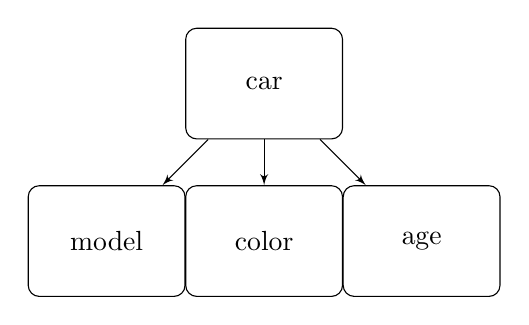
\begin{tikzpicture}[node distance = 2cm, auto]
% Place nodes
\node [block] (car) {car};
\node [block, below of=car] (color) {color};
\node [block, left of = color] (model) {model};
\node [block, right of = color] (age) {age};
\path [line] (car) -- (color);
\path [line] (car) -- (model);
\path [line] (car) -- (age);
\end{tikzpicture}
\end{center}

However, as nicely combinatorial as this makes the framing of the problem, some schema matchers do use other representational data besides what can be captured in such a model. For example, OntoBuilder \cite{ontobuilder}, which scrapes its schemas from website forms, uses the ordering of the form elements in the DOM structure of the forms to aid its matching process. For example, when extracting a schema about a trip, it is valuable to have the information that the ``depart date'' field comes before the ``return date'' field, since perhaps on a different webpage about the same information, they are called the ``leave date'' and the ``arrive date,'' making lexical comparisons difficult. 

Along the same lines, the situation is much changed if one deals with schemas which come from database specifications or similar, since in that case the volume of instance data will generally provide the most useful tool for matching. In particular, database table schemas will often lack pre-existing relational structure, being just a collection of columns, making the task of figuring out similarity one almost entirely coming from the format of the table contents. We will hence examine techniques for estimating similarity from instance data as their own category in the next section.

Auxiliary information to help matching can also be external to the data: when working in a well-traversed domain, semantic dictionaries are often valuable. This can be implemented as a third schema in addition to the two which are to be matched, which contains relevant items in the domain (and thus probably many of the items in the two schemas), in which all the real-world semantic relations are known. Such semantic dictionaries can be compiled independently of any schema matching, but previous schema matches from the same domain can also be used to generate approximations to dictionaries of this kind, which is often helpful when one is using a matcher many times on a project. This last idea in particular is one of the main features of COMA. As a simple example of this, two items in schemas labeled ``soccer'' and ``basketball'' might appear to have no relation based on only the schemas themselves, yet one might wish to know that they both areball sports, which could be accomplished if one had a third schema created from this real-world information.

\section{Item similarity}

As mentioned earlier, the primary way matches between schema items are found is via various ways of calculating similarity between each pair of items, one from the first and one from the second schema. These similarity measures can be roughly divided into three types: those using the item labels, those using the schema structure, and those using the instance data; we will give an account of some notable methods belonging to each type. 

In this section, we will by default assume that one is looking for simple two-way relationships rather than more complicated asymmetrical ones, since the idea of a coefficient of similarity is more naturally applicable to the former. However, similarity measures which may also be used asymmetrically will be noted as well when they appear.

An essential point to remember is that each of these methods outputs a numerical measure of similarity, generally normalized to a number between $0$ and $1$ for later aggregation purposes. For example, methods which simply look for the presence or absence of some feature common to both item labels may have some weight like $0.5$ or $0.7$ assigned to a successful match depending on how significant such a common feature is felt to be; these relative magnitudes may turn out to be significant later depending on the aggregation process used, though not if the measures are reweighted before aggregating (see next section). Thus, there is certainly a fair amount of arbitrariness involved.

Matching just by item label, of course, is the simplest class; the methods involved are just all the standard methods of finding similiarities between two strings. Such methods can be broadly divided into two subcategories of measures of lexicographic similarity (common substrings, edit distance, etc.) and semantic similarity, using a synonym/hyponym\footnote{A is a hyponym of B if every A is an B. One also says that B is a hypernym of A.} dictionary or similar auxiliary resource. Hyponyms and synonyms can be distinguished by assigning a hyponym relation a slightly lower coefficient than a synonym relation. For example, ``car'' and ``automobile'' might give a matching score of 0.7, whereas ``car'' and ``transportation'' only 0.5. Of course, in the asymmetrical case, a hyponym relation only will affect one of the two matching coefficients between the relevant items. 

Somewhat more refined than measures which just look at the labels of individual items are those which exploit the structure of the given schemas to some degree. Given graph representations, one can determine the lexical similarity of the labels of some set of ``relatives'' of a node, for example. In the case where the graphs are directed and so indicate a hierarchical relationship of concepts, this is especially useful, since one can compare the chains of parent nodes, or all the lowest-level children (``leaves''), which will tend to contain much semantic information. The OntoBuilder process mentioned in the previous section is also an example of a method of this type, as it uses the DOM hierarchy (which is even totally ordered) of the online forms from which it extracts the schemas in a similar way as described. For a simple example involving graph representations, suppose we have two schemas as follows:

\begin{center}
	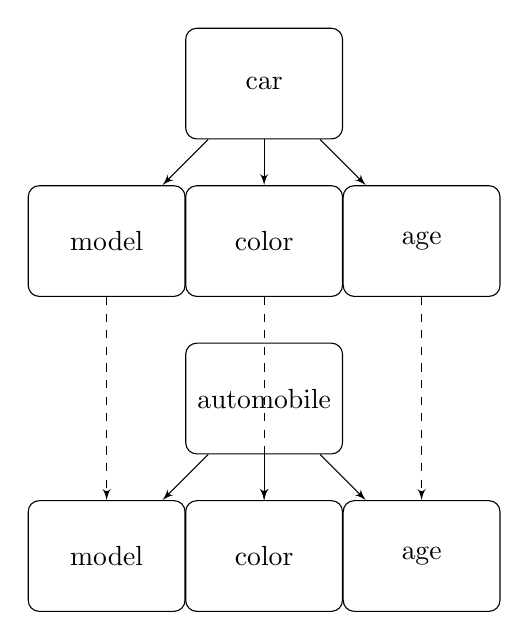
\begin{tikzpicture}[node distance = 2cm, auto]
	% Place nodes
	\node [block] (car) {car};
	\node [block, below of=car] (color) {color};
	\node [block, left of = color] (model) {model};
	\node [block, right of = color] (age) {age};
	\path [line] (car) -- (color);
	\path [line] (car) -- (model);
	\path [line] (car) -- (age);
	
	% Place nodes
	\node [block, below of = color] (automobile) {automobile};
	\node [block, below of=automobile] (color2) {color};
	\node [block, left of = color2] (model2) {model};
	\node [block, right of = color2] (age2) {age};
	\path [line] (automobile) -- (color2);
	\path [line] (automobile) -- (model2);
	\path [line] (automobile) -- (age2);
	
	\path [line,dashed] (color) -- (color2);
	\path [line,dashed] (age) -- (age2);
	\path [line,dashed] (model) -- (model2);
	\end{tikzpicture}
\end{center}

We can determine that ``car'' and ``automobile'' are the same without recourse to semantic methods, purely from the extreme similarity of their children.

Finally, there is measuring similarity based on instances. The obvious way to do this is just by applying an aggregate version of one of the similarity measures like those used for label names. For example, given a method to determine lexicographic similarity between any pair of instances, one can take an average of the similarity scores for the best match over every instance for one (or both) items. \cite{comainstance}

One can also exploit structural features of the instances. One method, described in \cite{regex}, is to develop a library of common formats (e.g. different ways to write dates/times, email addresses, zip codes, etc.) described by regular expressions, and assign higher similarity scores to pairs of items whose items match corresponding regex formats well. In some cases, like database specifications, some of this datatype information is actually encoded in the schema, and so that can simply be used instead.

Given a set of measures to use, a natural way to store all the obtained numerical similarities is in a matrix, in which rows correspond to items from one schema and columns to items from another; each measure then has its own matrix. (Alternately, it can be conceived of as a third dimension of the matrix; hence the term ``similarity cube'' used by \cite{coma}.) Such a matrix might look like the one below with two layers corresponding to two very simple matchers:

\begin{tabular}{|c|c|c|c|c|}
	\hline
LEXICAL & car & color & age & owned by \\\hline
automobile & 0 & 0 & 0 & 0 \\\hline
color & 0 & 1 & 0 & 0 \\\hline
years & 0 & 0 & 0 & 0 \\\hline
owner & 0 & 0 & 0 & 0.6 \\\hline
\end{tabular}

\begin{tabular}{|c|c|c|c|c|}
	\hline
	SEMANTIC & car & color & age & owned by \\\hline
	automobile & 0.9 & 0 & 0 & 0 \\\hline
	color & 0 & 1 & 0 & 0 \\\hline
	years & 0 & 0 & 0.4 & 0 \\\hline
	owner & 0 & 0 & 0 & 0.5 \\\hline
\end{tabular}


Before aggregation, however, often it is useful to do some ``post-processing'' of the similarity matrix, as similarity scores between items can be used in conjunction with other ideas to obtain better measures. For example, if our schemas are directed graphs indicating a hierarchical relation, items/nodes whose children have strong similarity scores should also obtain a boost to their own similarity scores. This is especially relevant if child nodes are the ones with instance data, and so can be analyzed for similarity more thoroughly, since this gives us a way to pass that information back up the tree; see \cite{comainstance}. 

In addition, one may wish to assume transivity in matching; if the edges in a graph representation are bidirectional and indicate some sort of relatedness, matching scores can be propagated in those directions. If one uses an intermediary schema containing already known semantic information, as suggested earlier, this type of propagation can also be used.

\section{Aggregation}

Before aggregating all of the individual similarity scores into actual matches between schema items, one must decide whether one wishes to do a left merge or a total merge. That is, does one want the final schema to essentially be the left schema with as much of the right schema integrated as possible, or a collection of all items in both schemas, with some items identified? The two make sense in different contexts, though the tools we will describe below are not substantially different between them.

\cite{coma} breaks down the progression to selecting matches based on the matrix of similarity scores in a very logical fashion, so I follow them here. 

In the first place, one should calculate an aggregate score for each pair of items, based on all of the match scores (as well as any auxiliary/derived scores, as mentioned at the end of the last section). Conceptually, this is just some sort of measure of center of all of the similarity scores. On one extreme, we can be very risky and take the maximum similarity score; this is almost never a good idea, especially since many of the individual matchers mentioned above are very naive and shallow on their own. On the other, we can be extremely conservative and take the minimum score; this is also usually ill-advised. In between, there are averages of all kinds, the simplest of which would be the classic unweighted mean and median. 

Weighted averages offer more sophistication, and indeed, simply putting weights on matchers based on heuristic estimates of how reliable they are can be useful. Even more effective, however, is the idea of using machine learning. With a relatively small amount user input in the form of some number of true item matches, matching algorithms such as LSD \cite{machine} use the performance of different matchers on this training data to find appropriate weights. (Various algorithms can be used; LSD simply does a least squares regression.) 

To fine tune this further, one could adopt an idea implemented in DataMade's Dedupe algorithm, for the related problem of finding duplicate rows in a database: using the matchers, create an initial model of matches between the schemas, and then solicit input from the user by asking about whether certain items are true matches so as to adjust the weights as efficiently as possible.

Given now a way to obtain aggregate match scores between each pair of items (i.e. having collapsed the third dimension of the similarity cube), it remains to actually select the match candidates. One can require the candidate to be the best match for each item in the first schema, the best item for each item in the second schema, or both, depending on how conservative one wishes to be. In the case of a left merge, of course only the first and the third options make sense.

If one wishes to potentially allow multiple matches, one can use some combination of setting an absolute threshold and choosing top-$n$ matches. An interesting idea from \cite{coma} is to set a threshold relative to the score of the best match, the idea being that multiple matches should occur when there is a group of potential matches which all have close to the same high score.

\section{Evaluation}

With artificially chosen examples of a certain type, evaluation of schema matching can be done in a perfectly standard way. That is, evaluating on schemas which are small and simple enough that objectively correct matches can be given by hand, one can evaluate a schema matcher simply by using the standard measures of precision and recall of automatically detected matches against true matches, inside the space of all possible matches between items.

However, behavior on problems which are larger and more complex may be drastically different than the simple ones for which this is possible; such problems not only may not be feasible to do by hand, but may not have a clear objectively correct set of matches. One would also like to get an idea of how effective a ``real'' application of the matching is, which of course is not hand-verifiable, since otherwise there is no need for the tool. Furthermore, the above discussion on precision/recall applies naturally only to total merges.

To this end, \cite{comabenchmark} outlines some measures which can be used to judge the quality of a matching by means other than accuracy relative to some ``true'' set of matches. Instead, the measures evaluate other aspects of the quality of the merge, based on conceptual understandability and coherence. The essential concepts used are those of coverage, redundancy, compactness.

The \textbf{coverage} of a match refers to what ratio of the total combined items of the original two schemas are represented in the final schema. In cases where the schemas are inheritance-type structures (i.e. represented by directed graphs), particularly when only the bottom-level child items have instance data associated with them like in many databases, one may also consider this ratio restricted to these bottom-level items, since the idea here is that we do not wish to lose information. Of course, this only really makes sense either when we are doing a left merge, or when we are using a match candidate selection technique (see previous section) involving thresholding of some sort; otherwise, of course all the items will be included and the result will always be $1$.

The \textbf{compactness} of a match refers to the ratio of the size of the final merged schema to the sum of the sizes of the two schemas individually. A lower number is desirable because, often, one of the points of the merge is to reduce the schema to a more humanly comprehensible size.

The \textbf{redundancy} of a match applies in cases of inheritance-type directed graph representations; the idea is that one would not like the bottom-level child items to have multiple inheritance paths. Thus, we define it as the ratio between the number of inheritance paths to bottom-level items in the final merged schema to the number of bottom-level items.

Clearly, much like traditional measures such as precision/recall, these measures are designed to have mutual trade-off relationships. For example, coverage and compactness obviously are mutually antagonistic; the only way to obtain both is to match a very high number of items. One can think of redundancy as a measure to prevent just blindly matching many items to achieve good coverage and compactness, since if many of the matches were spurious, almost certainly the non-matching inheritance structures would cause a great deal of redundancy.

\section{Further resources}

It shoudld be noted that the literature on schema matching/ontology merging is vast, and this article did not begin to review it. Instead, aiming at giving an idea of the different steps in how a matching algorithm might be implemented, it largely followed the outline of one particularly flexible matcher (COMA) with many common features. An enormous number of other matchers exist, however, some having completely different sets of features.

A much more comprehensive further resource is \url{ontologymatching.org}, the home page of an organization which hosts academic conferences on the topic. There, one can find much more comprehensive (though often extremely long) surveys, other recent publications, and information on conferences. A subsidiary, the Ontology Alignment Evaluation Initiative, documents online its evaluations of many existing matchers, which may also be of interest.

Finally, listed below are a collection of open-source schema matchers whose licensing, documentation, and source code is all easily accessible online. A brief summary of their basic features is given in the table, though of course each also has many other varying focuses and strengths.

\begin{tabular}{|c|c|c|c|c|c|}
\hline
& COMA 3.0 & OntoBuilder & AgreementMaker & LogMap & S-Match \\\hline
Custom matchers & Yes & Yes & No & No & No \\\hline
Instance data & Yes & Yes & No & No & No \\\hline
Machine learning features & No & No & No & Yes & No \\\hline
Semantic learning features & Yes & No & Yes & Yes & Yes \\\hline
\end{tabular}

These matchers can be found at the following URLs:
\begin{itemize}
\item COMA: \url{http://dbs.uni-leipzig.de/de/Research/coma.html}
\item OntoBuilder: \url{https://bitbucket.org/tomers77/ontobuilder/wiki/OntoM}
\item AgreementMaker: \url{https://agreementmaker.github.io/}
\item LogMap: \url{https://www.cs.ox.ac.uk/isg/tools/LogMap/}
\item S-Match: \url{http://semanticmatching.org/s-match.html}
\end{itemize}

All matchers listed are cross-platform, written in Java, with both command-line and graphical interfaces. They all accept inputs via the standard XML-based format OWL specified by W3C, though other formats are supported by some. 

\begin{thebibliography}{9}
	\bibitem{comasemantic}
	Arnold, Patrick and Rahm, Erhard.
	``Enriching Ontology Mappings with Semantic Relations.''
	University of Leipzig.
	\url{http://dbs.uni-leipzig.de/file/document_0.pdf}	

	\bibitem{coma++}
	Aumuller, David et. al.
	``Schema and Ontology Matching with COMA++.''
	\emph{SIGMOD 2005} (June 2005). 
	\url{http://dbs.uni-leipzig.de/file/comaplusplus.pdf}
	
	\bibitem{coma}
	Do, Hong-Hai and Rahm, Erhard.
	``COMA - A system for flexible combination of schema matching approaches.''
	\emph{Proceedings of the 28th VLDB Conference}, Hong Kong (2002).
	\url{dbs.uni-leipzig.de/file/COMA.pdf}
	
	\bibitem{machine}
	Doan, AnHai et. al.
	``Reconciling Schemas of Disparate Data Sources: A Machine-Learning Approach.''
	\emph{ACM SIGMOD}, Santa Barbara (2001).
	\url{http://homes.cs.washington.edu/~pedrod/papers/sigmod01.pdf}
	
	\bibitem{comainstance}
	Engmann, Daniel and Massmann, Sabine.
	``Instance Matching with COMA++.''
	University of Leipzig.
	\url{ http://dbs.uni-leipzig.de/file/BTW-Workshop_2007_EngmannMassmann.pdf}
	
	\bibitem{ontobuilder}
	Gal, Avigdor and Modica, Giovanni.
	``Onto-Builder: Fully Automatic Extraction and Consolidation of Ontologies from Web Sources.''
	\url{http://ceur-ws.org/Vol-82/SI_demo_04.pdf}

	\bibitem{comabenchmark}
	Raunich, Salvatore and Rahm, Erhard.
	``Towards a Benchmark for Ontology Merging.''
	University of Leipzig.
	\url{http://dbs.uni-leipzig.de/file/E2IN2012-raunich-rahm.pdf}

	\bibitem{regex}
	Zapilko, Benjamin et. al. 
	``Utilizing Regular Expressions for Instance-Based Schema Matching.''
	Leibniz Institute for the Social Sciences.
	\url{http://ceur-ws.org/Vol-946/om2012_poster4.pdf}
\end{thebibliography}
\end{document}